

%%
%% File: test-02.tex
%% Tests xlayout for scrbook class.
%% 26/05/2012
%%
%%
\documentclass[twoside,10pt]{scrbook}
\usepackage{tikz,changepage,fancyhdr,amsmath}
\usepgflibrary{arrows}
\usepackage{lipsum}
\uspackage[german]{babel}
\usepackage[german]{xlayouts}
\renewcommand{\topfraction}{.6}
\renewcommand{\bottomfraction}{.8}
\renewcommand{\textfraction}{.04}
\renewcommand{\floatpagefraction}{.9} % have a high one don't encourage it
\renewcommand{\dbltopfraction}{.5}
\renewcommand{\dblfloatpagefraction}{.8}
\setcounter{topnumber}{9}
\setcounter{bottomnumber}{9}
\setcounter{totalnumber}{2}
\setcounter{dbltopnumber}{1}
\pagestyle{grid}
\begin{document}
\section{Introduction}
\thispagestyle{grid}
\begin{figure}[b]
\ifbotfloat{\figureparamsbot}{%
 \iftopfloat{\figureparamstop}{}}

\centering
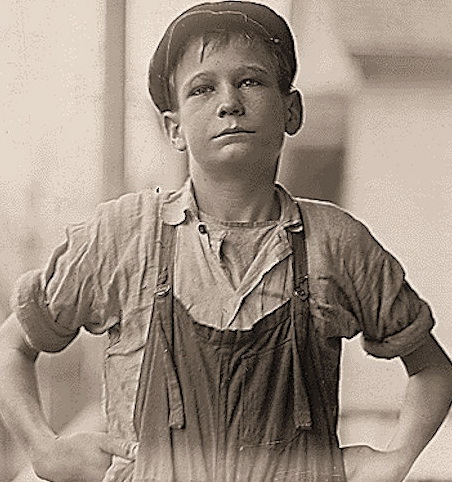
\includegraphics[height=0.9\columnwidth]{./images/hine04-x}
\caption{Example image to demonstrate top fraction.}
\end{figure}
\lipsum[1]

\lipsum[1]

This has been drawn using TikZ\footnote{A kleine program.}\footnote{Another footnote.}.
\lipsum[1-2]
\begin{figure}[t]
 \caption{Example image to demonstrate top.}
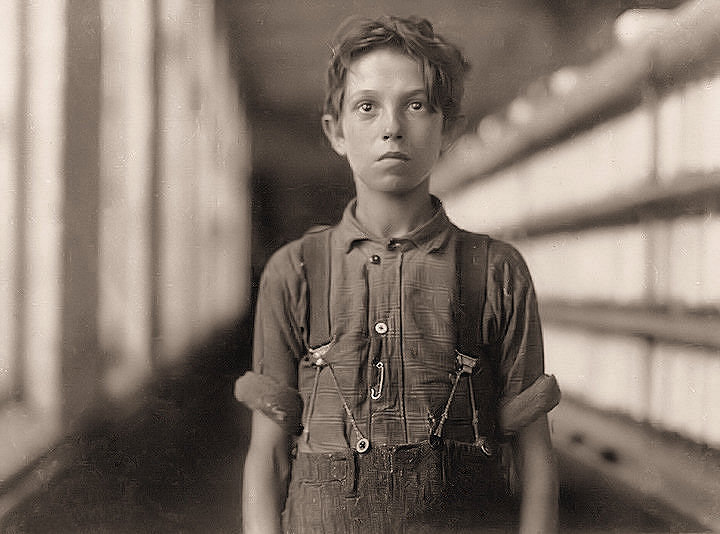
\includegraphics[width=\columnwidth]{./images/hine02}%
  \iftopfloat{\figureparamstop}{}
\end{figure}
\begin{figure}[tpb]
\centering
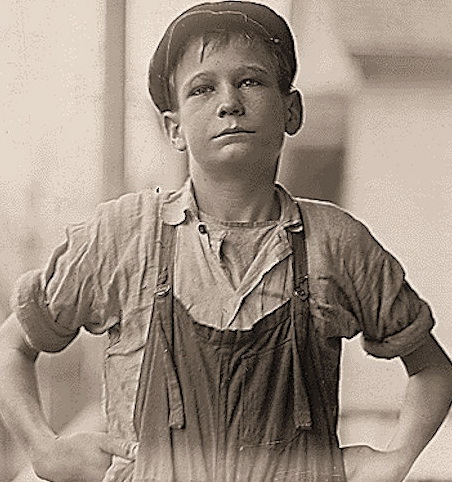
\includegraphics[height=\columnwidth]{./images/hine04-x}
\caption{Example image to demonstrate top fraction.}
\end{figure}

\begin{figure}[tpb]
\centering
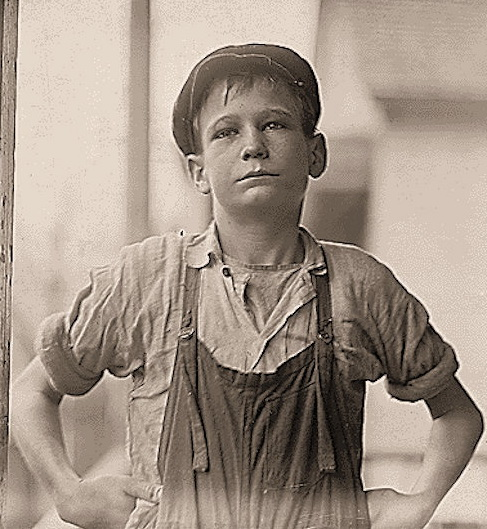
\includegraphics[width=\columnwidth]{./images/hine04-xx}
\caption{Example image to demonstrate top fraction.}
\end{figure}
\lipsum
\clearpage
\onecolumn
\drawcanons

\printreadability
\pagestyle{plain}
\newpage
\drawtriallayout
\newpage
\drawtriallayout
\end{document}



